% stato della relazione :
%
%AMMERDAAAAAAAA
%
\documentclass[a4paper,twoside]{article}

\usepackage[margin=3cm]{geometry}
\usepackage[utf8]{inputenc}
\usepackage[main=italian, english]{babel}
\usepackage{graphicx}
\usepackage{rotating}
\usepackage{verbatim}
\usepackage{listings}
\usepackage[colorlinks=true,linkcolor=black,urlcolor=blue]{hyperref} % ancore delle varie sezioni sul menu
\usepackage{float}

%\graphicspath{Immagini/} non funziona

\author{Giuseppe Merlino, Miki Violetto}
\title{Relazione progetto BiciRent}
\date{\today}

\begin{document}
\maketitle

\newpage
\tableofcontents
\newpage
\listoffigures
\newpage

\section{Abstract}
BiciRent è un servizio di bike sharing ispirato a Goodbike presente qui a Padova.\newline
Permette il noleggio di biciclette da utilizzare per girare per la città grazie a delle tessere personali e grazie a molte stazioni dislocate su varie aree della città è possibile prelevare e depositare la bicicletta con comodità.\newline
Il progetto si focalizza sulla gestione dei noleggi e delle operazioni di routine eseguibili dall'utenza e dai tecnici di BiciRent, virtualizzando su un sito le operazioni che verrebbero normalmente svolte su vari dipositivi come le colonnine, un'applicazione per gli utenti o una per i tecnici.
\section{Descrizione testuale dei requisiti e operazioni tipiche}
\subsection{Descrizione testuale}
Al momento dell'iscrizione di un utente verranno richiesti tutti i dati personali necessari a registrarlo e rilasciarli la tessera, quali nome, cognome, data e luogo di nascita, infomazioni sulla residenza, e un'email quale recapito per essere contattato; grazie a queste informazioni gli verrà rilasciata una tessera personale con la quale utilizzare tutti i servizi, e avente una validità definita dal piano  che è stato scelto.\newline
A seconda del piano ci sono varie agevolazioni per i turisti e gli studenti, i quali però dovranno dimostrare di esserlo con la matricola universitaria o la carta IoStudio; il sito non si preoccupa di permettere l'acquisto o l'aggiornamento di questi piani, ma svolge solo un'azione di deposito dei dati, e controllando se l'utente utilizza una tessera con un piano scaduto.\newline
Un utente potrà quindi prelevare una bicicletta da una colonnina di una stazione e poi depositarla su una qualsiasi colonnina libera: queste operazioni, chiamate prelievo e deposito, dovranno venire registrate dal sito con in aggiunta l'orario in cui vengono effettuate.\newline
Sia le biciclette che le colonnine sono dei beni identificati da un codice comune che identifica tutti i beni dell'azienda BiciRent, inoltre questi materiali possono essere danneggiati: un materiale danneggiato non permette alcuna operazione su di esso da parte dell'utente e deve venire riparato dai tecnici.\newline
Deve venire registrata ogni riparazione eseguita dai tecnici, con in aggiunta una descrizione del danno riparato.\newline
Le biciclette possono essere a pedalata assistita (elettriche) oppure a pedalata normale e possono essere in servizio (cioè ferme nelle colonnine oppure nolleggiate) o in magazzino; una bicicletta danneggiata può ovviamente essere sia in magazzino che in una colonnina.\newline
Le colonnine sono presenti in gruppi su tutto il territorio, raggrupate in stazioni che vengono identificate dal loro indirizzo, e possono essere libere oppure occupate da una bicicletta. Una colonnina danneggiata rende la bicicletta (se presente) danneggiata anch'essa.\newline
Ulteriori informazioni che devono essere registrate sono le segnalazioni da parte dell'utente e le informazioni relative ai trasporti eseguiti dai tecnici.\newline
Un utente può segnalare una mancanza su una stazione, cioè se vuole eseguire un noleggio (o un deposito) e la stazione ha tutte le colonnine vuote (o occupate) può segnalare questo ai tecnici; allo stesso modo può segnalare una reottura su una colonnina ( e sulla bicicletta presente quindi).\newline
I trasporti eseguiti dai tecnici sono del tutto simili alle operazioni eseguite dai clienti, solo che l'aggiunta o rimozione di una bicicletta può essere eseguita solo dai tecnici, mentre il noleggio e il deposito solo dai clienti muniti di tessera, ma non si vuole tener traccia del tecnico.\newline
Il sito dovrà virtualizzare le operazioni che normalmente un cliente esegue su una colonnina, quindi un prelievo di una bicicletta passando la sua tessera, o un deposito, o una segnalazione di rottura (eseguita su una colonnina, per questo non si discrimina se è la bicicletta o la colonnina); dovrà inoltre prevedere un'area in cui è possibile per l'utente controllare i suoi noleggi, i suoi dati personali e lo stato delle stazioni ( nella realtà queste informazioni gli sono accessibili tramite un'applicazione per smartphone). Inoltre dovrà esserci un'area amministrativa in cui i tecnici possono registrare le manutenzioni che fanno e controllare le segnalazioni eseguite dagli utenti.\newline
Alcune informazioni di traffico previsto: si prospettano circa 1700 noleggi giornalieri e una media di 200 richieste d'intervento al giorno (mancanza di bici e rotture); inoltre viene richiesta la composizione dei posti delle stazioni (presenza biciclette, tipi disponibili e posti liberi) almeno 10000 volte ogni giorno, ma con punte di quasi 900 richieste in una singola mezz'ora (ad esempio nelle ore di punta).
\section{Progettazione concettuale}
Per la modellazione concettuale si decide di utilizzare un metodo misto e partire dal'operazione di noleggio.\newline
Il noleggio è formato da due distinte operazioni, un prelievo che inizia il noleggio, e un deposito che lo termina; il deposito distingue inoltre il noleggio pendente, cioè non ancora terminato, con il noleggio terminato il quale è anche uno storico dei noleggi.
\begin{figure}[H]
 \centering
  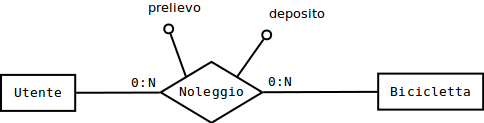
\includegraphics[width=1\textwidth]{Immagini-Grafici/Concettuale01.png}
\caption{Relazione Noleggio}
\end{figure}
Le informazioni personali dell'utente vengono rappresentate con l'entità Utente; Studente e Turista sono specializzazioni parziali esclusive; l'utente viene identificato dalla tessera che possiede e utilizza nel sito.
\begin{figure}[H]
 \centering
  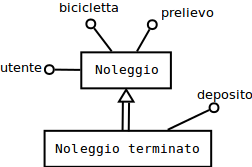
\includegraphics[width=1\textwidth]{Immagini-Grafici/Concettuale02.png}
\caption{Entità utente}
\end{figure}
\begin{figure}[H]
 \centering
  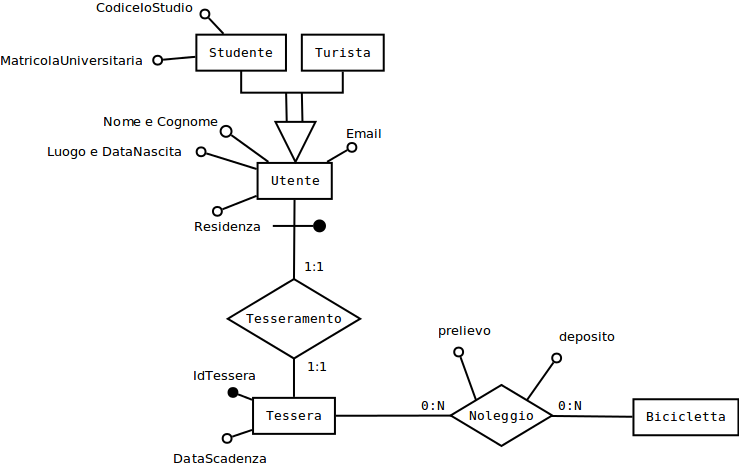
\includegraphics[width=1\textwidth]{Immagini-Grafici/Concettuale03.png}
\caption{Relazione Noleggio}
\end{figure}
La informazioni di tessera non possono essere rappresentate da un singolo attributo, quindi lo si reifica in un'entità.
\begin{figure}[H]
 \centering
  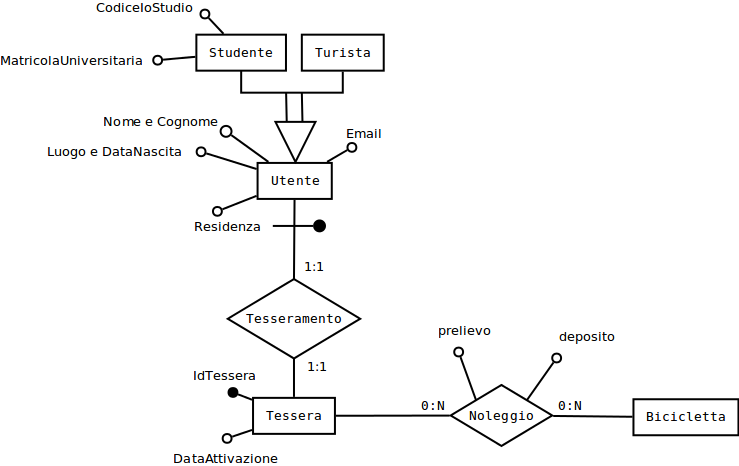
\includegraphics[width=1\textwidth]{Immagini-Grafici/Concettuale04.png}
\caption{Entità Tessera}
\end{figure}
Le informazioni della bicicletta vengono rappresentate dall'entità Bicicletta, identificata dal codice del materiale.
\begin{figure}[H]
 \centering
  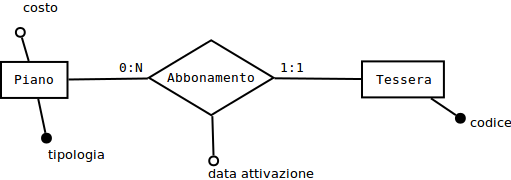
\includegraphics[width=1\textwidth]{Immagini-Grafici/Concettuale05.png}
\caption{Entità Bicicletta}
\end{figure}
Sia prelievo che deposito sono un'operazione, che ha degli attributi propri.
\begin{figure}[H]
 \centering
  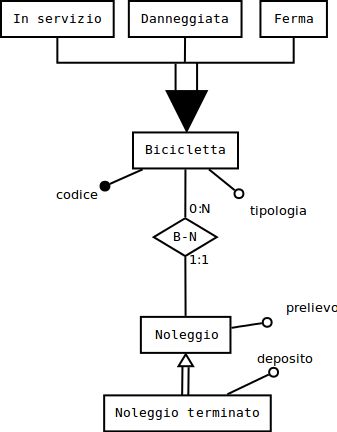
\includegraphics[width=1\textwidth]{Immagini-Grafici/Concettuale06.png}
\caption{Entità Operazione}
\end{figure}
Quindi la relazione noleggio scompare, essendo divisa in due relazioni che legano Tessera ad Operazione. Operazione inoltre contiene operazioni di trasporto.
\begin{figure}[H]
 \centering
  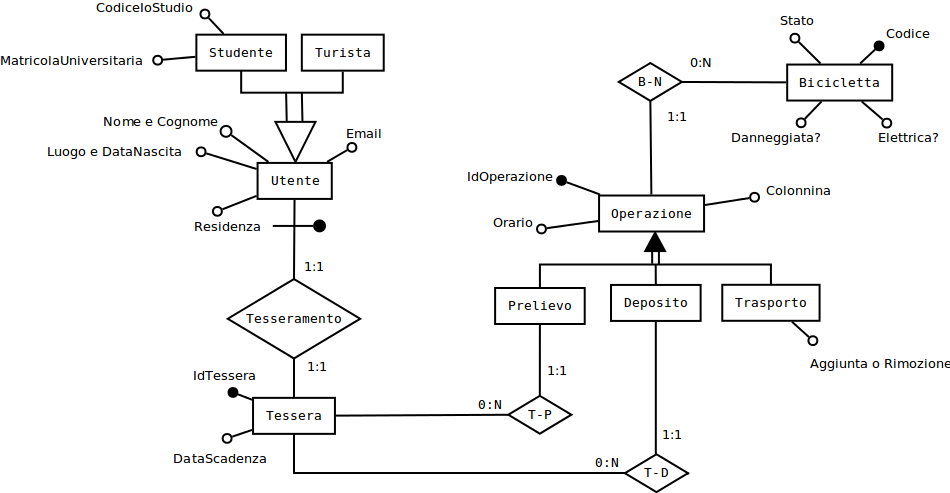
\includegraphics[width=1\textwidth]{Immagini-Grafici/Concettuale07.png}
\caption{Scomparsa della relazione Noleggio}
\end{figure}
La colonnina non può essere rappresentata da un solo attributo.
\begin{figure}[H]
 \centering
  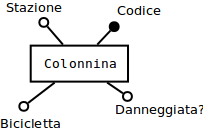
\includegraphics[width=1\textwidth]{Immagini-Grafici/Concettuale08.png}
\caption{Entità Colonnina}
\end{figure}
Per rappresentare la posizione di una Bicicletta su una Colonnina si utilizza una relazione.
\begin{figure}[H]
 \centering
  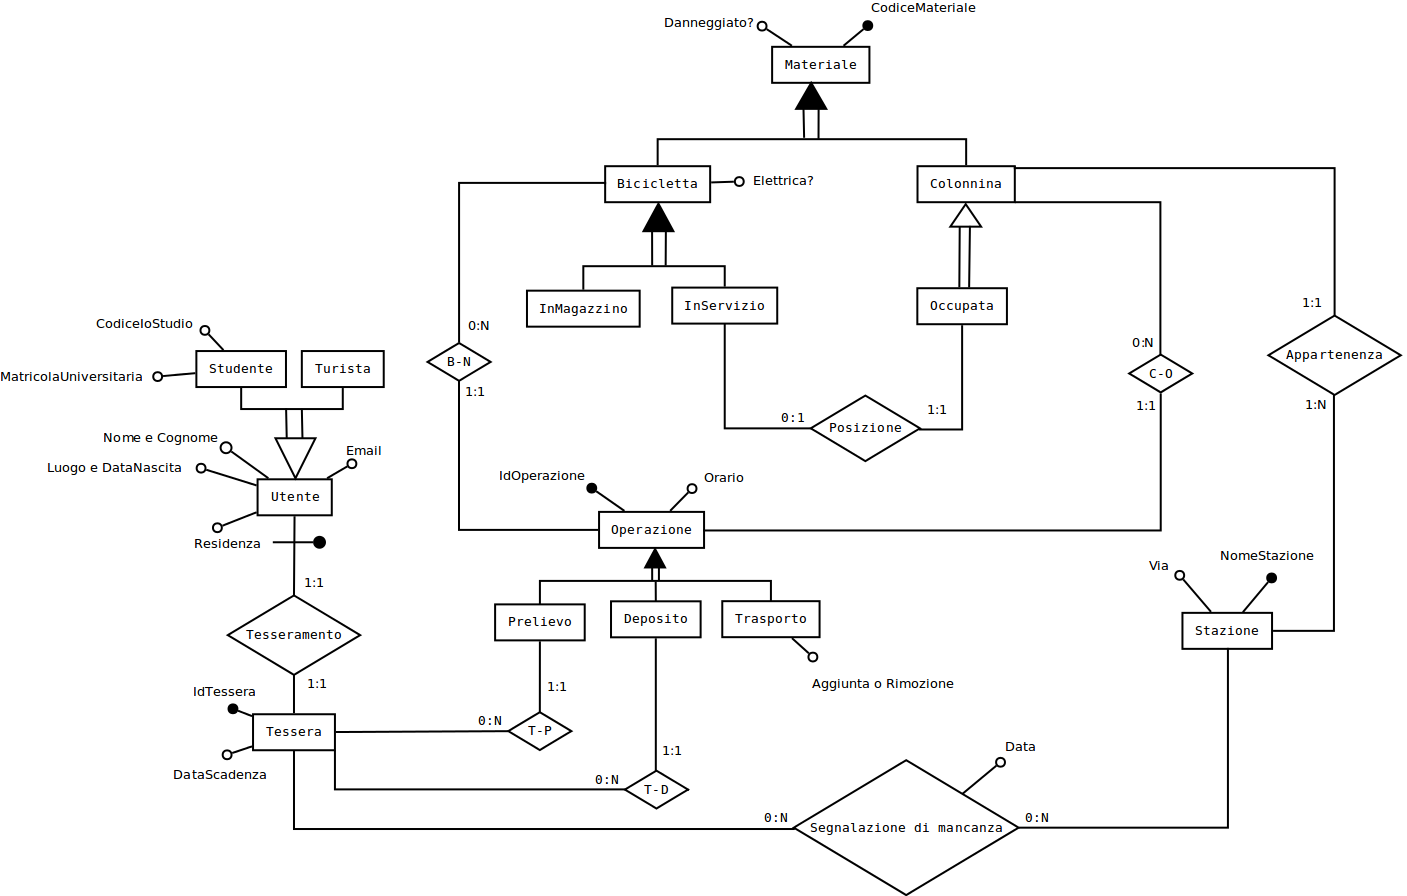
\includegraphics[width=1\textwidth]{Immagini-Grafici/Concettuale09.png}
\caption{Relazione Posizione}
\end{figure}
Quindi lo schema tra Operazione, Bicicletta e Colonnna è il seguente.
\begin{figure}[H]
 \centering
  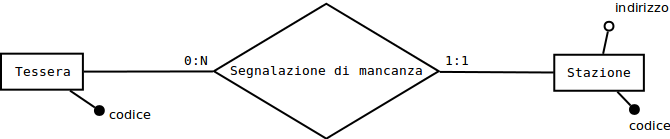
\includegraphics[width=1\textwidth]{Immagini-Grafici/Concettuale10.png}
\caption{Operazione, Bicicletta, Colonnina}
\end{figure}
Le colonnine sono raggruppate in Stazioni.
\begin{figure}[H]
 \centering
  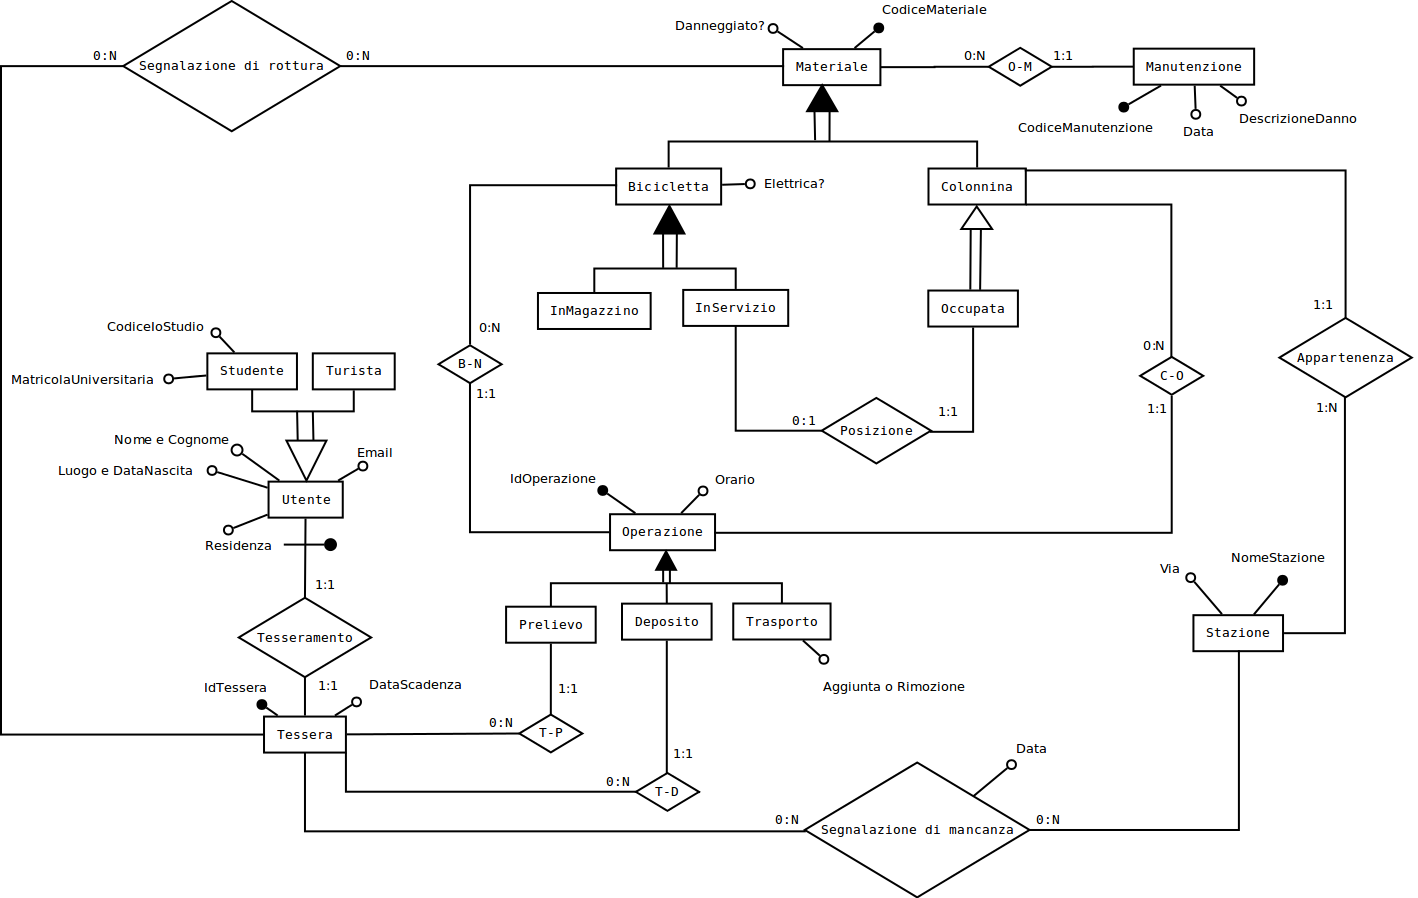
\includegraphics[width=1\textwidth]{Immagini-Grafici/Concettuale11.png}
\caption{Entità Stazione}
\end{figure}
Come descritto dai requisiti, sia le Colonnine che le Biciclette sono dei materiali, quindi sono specializzazioni complete ed esclusive
\begin{figure}[H]
 \centering
  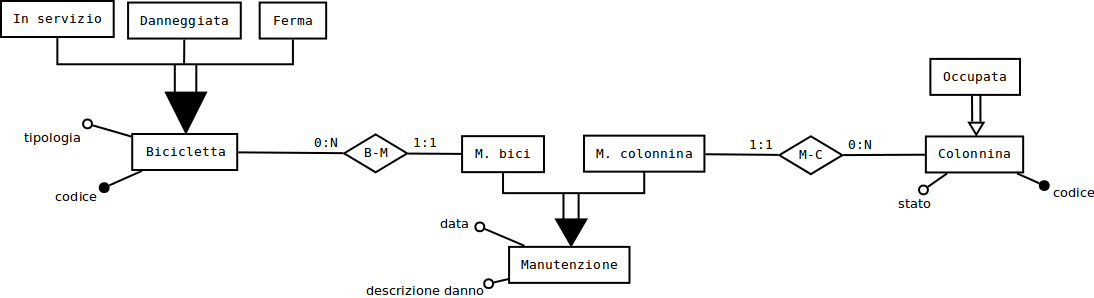
\includegraphics[width=1\textwidth]{Immagini-Grafici/Concettuale12.png}
\caption{Entità Materiale}
\end{figure}
\begin{figure}[H]
 \centering
  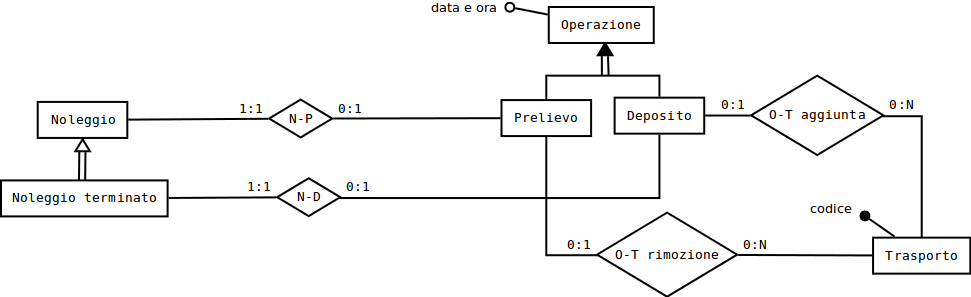
\includegraphics[width=1\textwidth]{Immagini-Grafici/Concettuale13.png}
\caption{Stato dell'Entità Materiale}
\end{figure}
Le segnalazioni di mancanza e di rottura vengono realizzata tramite delle relazioni.
\begin{figure}[H]
 \centering
  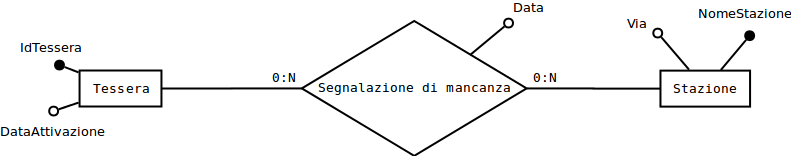
\includegraphics[width=1\textwidth]{Immagini-Grafici/Concettuale14.png}
\caption{Relazione Segnalazione di Mancanza}
\end{figure}
\begin{figure}[H]
 \centering
  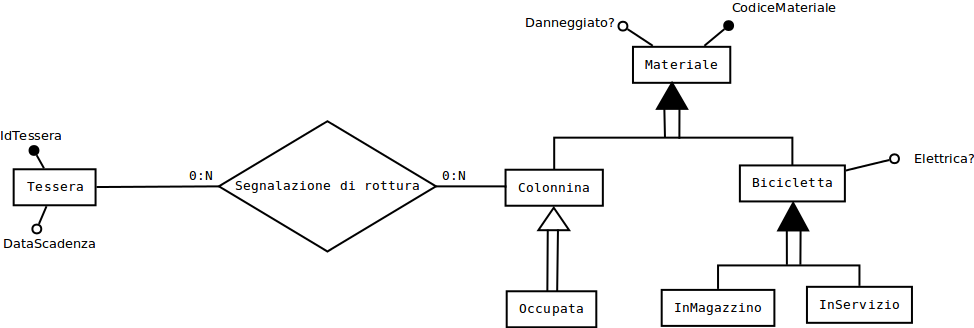
\includegraphics[width=1\textwidth]{Immagini-Grafici/Concettuale15.png}
\caption{Relazione Segnalazione di Rottura}
\end{figure}
Questo è il modello concettuale risultante.
\begin{figure}[H]
 \centering
  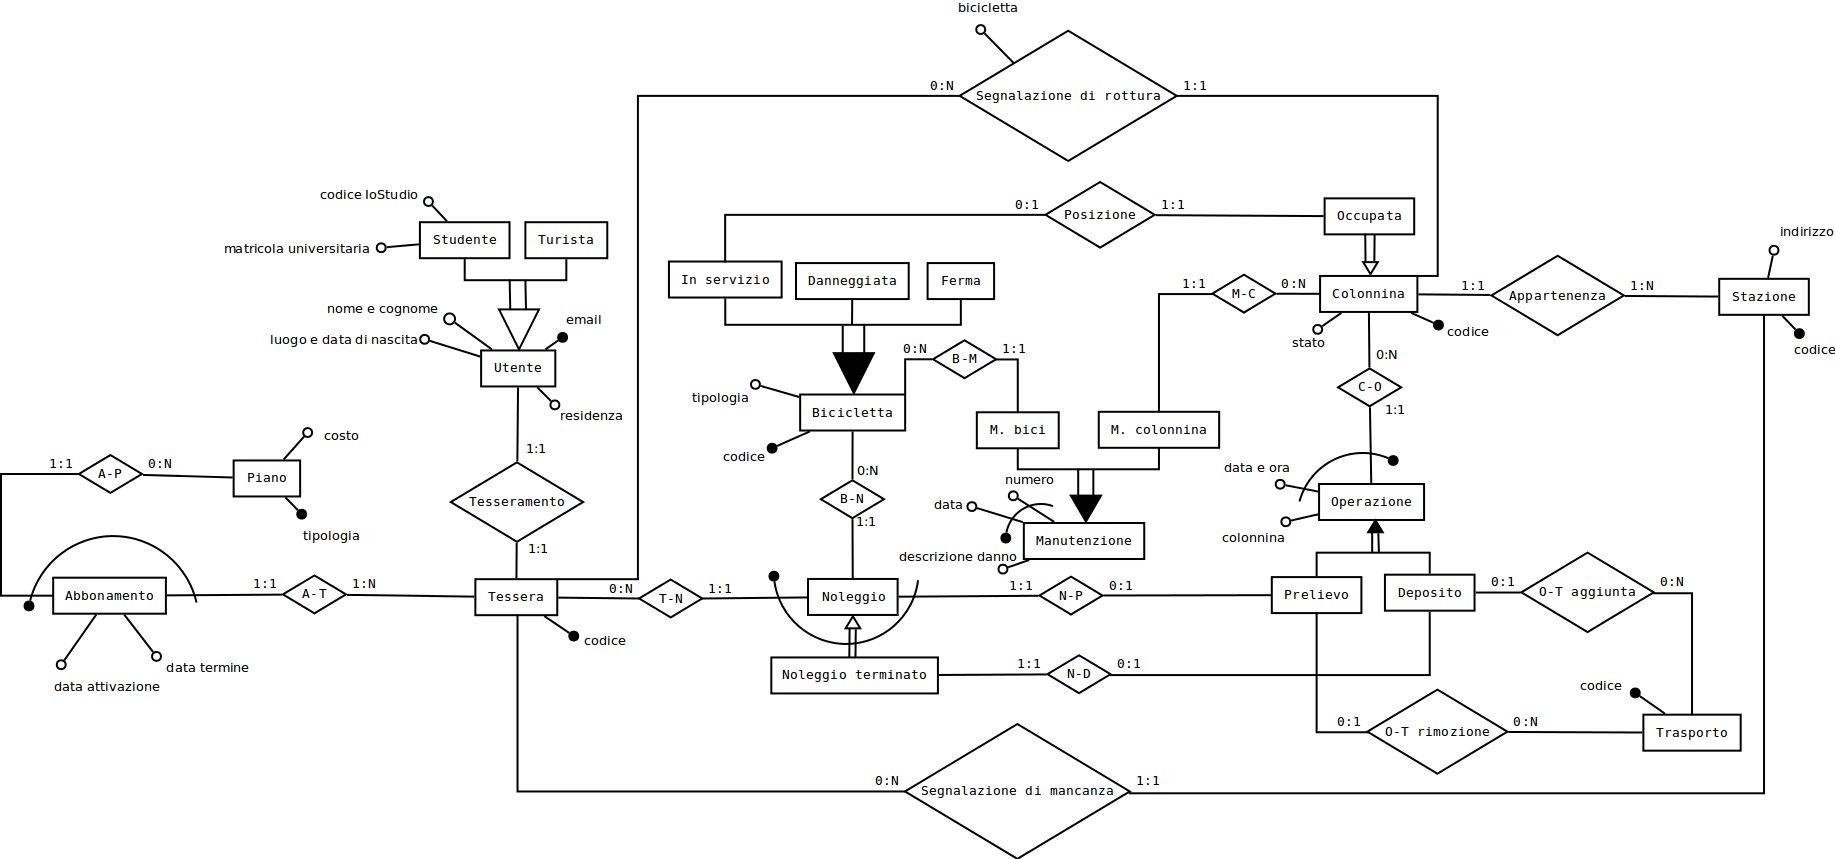
\includegraphics[width=1\textwidth]{Immagini-Grafici/ConcettualeFinale.png}
\caption{Modello Concettuale Finale}
\end{figure}
\section{Progettazione logica}
Per la realizzazione di un modello logico a partire da uno concettuale si sevono controllare varie cose:\newline
Per prima cosa si controllano le chiavi di ogni entità, e sono presenti tutte.\newline
Osservando Utente e Tessera si nota che hanno la stessa chiave, quindi le due entità potrebbero essere unite in un'unica, ma si decide di non farlo in quanto le informazioni dell'utente non vengono quasi mai richiamate (solo se si deve mostrare il profilo) e quindi avere una grande entità coinvolta in tutte le relazioni di tessera rallenterebbe inutilmente il sistema,molto meglio eseguire un join quelle rare volte che servono le informazioni personali dell'utente.\newline
Osservando ora Operazione, ci si accorge come i sottoinsiemi prelievo e deposito siano molto simili, quindi si decide di unirli in un unico sottoinsieme, e distinguerli grazie ad un attributo.\newline
Si osserva come Trasporto e Noleggio siano molto simili, ma al momento si preferisce aspettare all'implementazione su sql per decidere come comportarsi.
\begin{figure}[H]
 \centering
  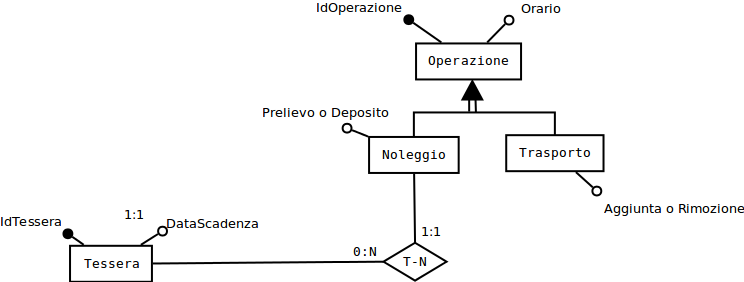
\includegraphics[width=1\textwidth]{Immagini-Grafici/Logico01.png}
\caption{Modifica a Operazione}
\end{figure}
Lo schema Logico risultate.
\begin{figure}[H]
 \centering
  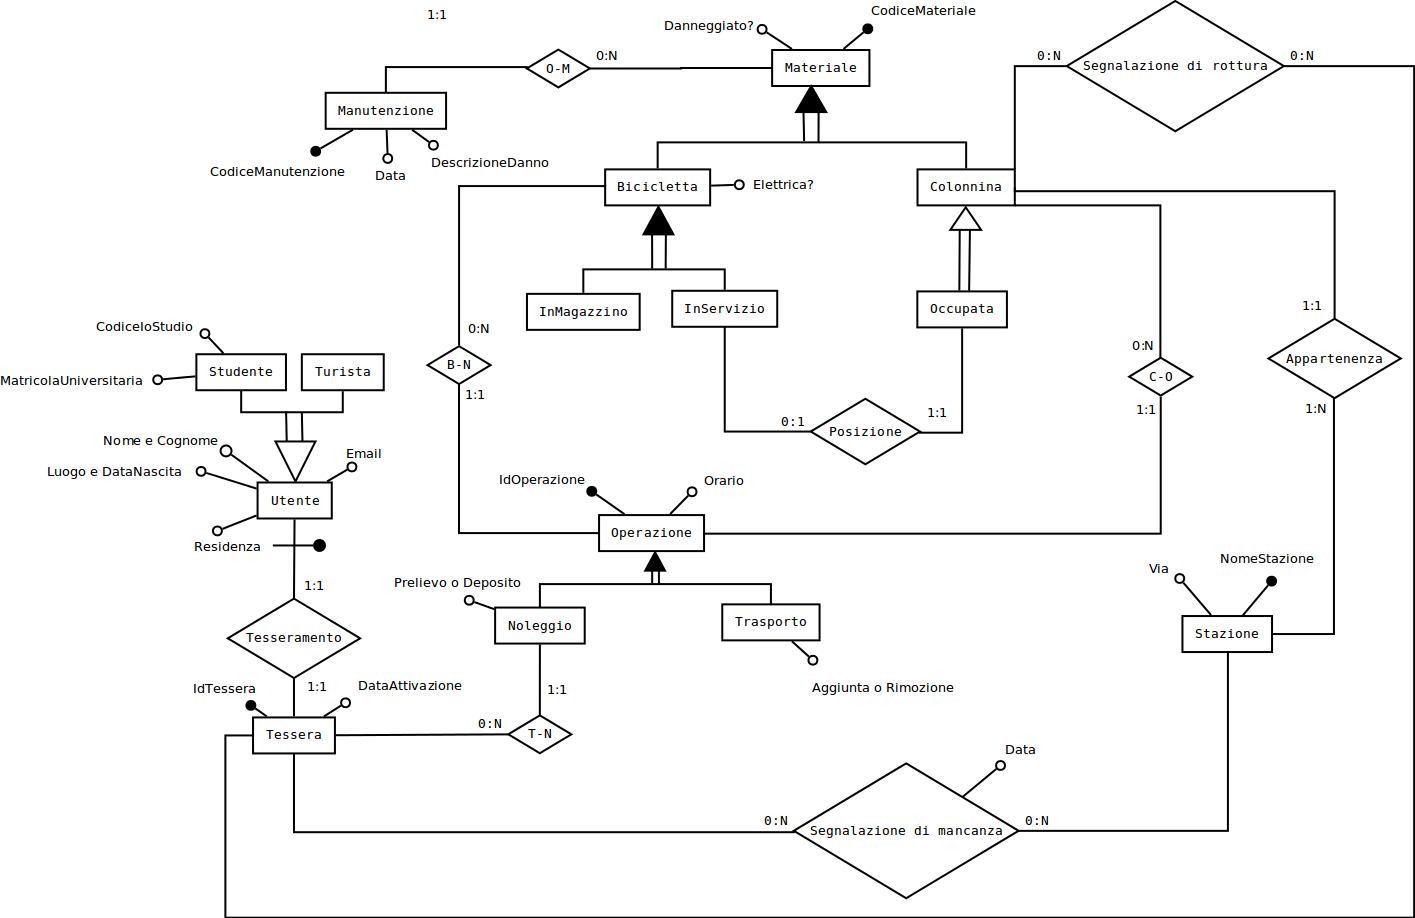
\includegraphics[width=1\textwidth]{Immagini-Grafici/LogicoFinale.png}
\caption{Modello Logico Finale}
\end{figure}
\section{Implementazione dello schema logico}
\subsection{Conversione iniziale}
Implementando lo schema logico con mysql si modificano varie parti dello schema Logico.\newline
Una prima conversione risultante dall'eliminazione delle relazioni tra le entità, rapprentate con l'aggiunta delle chiavi esterne: Segnalazione di Mancanza e Segnalazione di Rottura diventano entità (in quanto relazioni N:N).\newline
Inoltre si compiono varie scelte su come rappresentare i sottoinsiemi delle entità:
\begin{itemize}
 \item per Operazione, Bicicletta, Utente, e Colonnina si sceglie di compattare il tutto nell'entità e di aggiungere degli attributi di controllo, su cui sarà però necessario dei trigger o controlli aggiuntivi
 \item per Materiale si sceglie invece di creare 2 entità aggiuntive, in quanto sarebbe sennò stato necessario una serie di controlli complicati e un rallentamento non indifferente del sistema.
\end{itemize}
\begin{figure}[H]
 \centering
  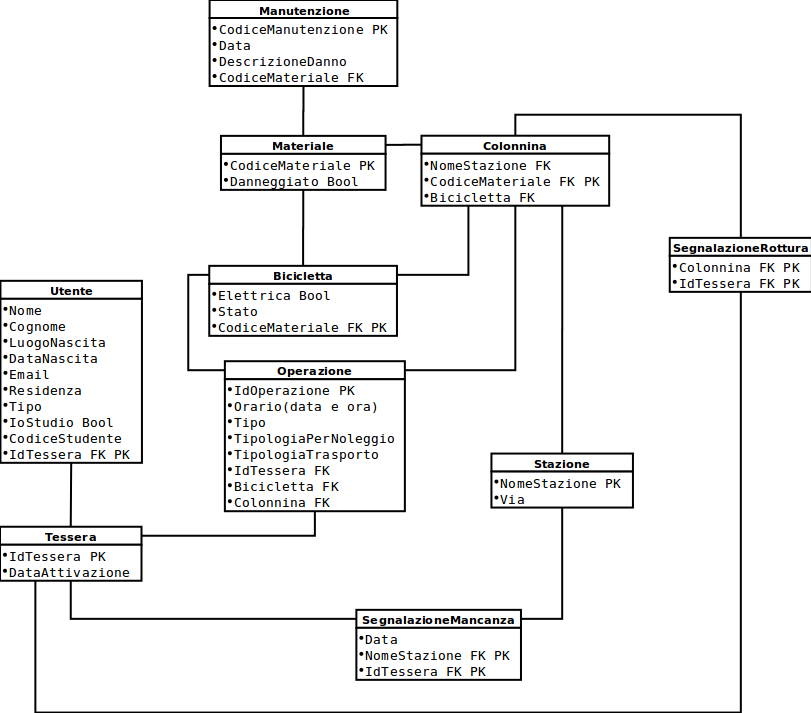
\includegraphics[width=1\textwidth]{Immagini-Grafici/SQL.png}
\caption{Trasformazione in sql}
\end{figure}
\subsection{Codice sql}
Si decide di implementare i controlli sono sulle operazioni che verranno effettivamente eseguite (non ci si preoccupa ad esempio della modifica della chiave primaria di materiale, perchè non viene permesso di farlo).\newline
Tessera
\begin{lstlisting}[ language=SQL, showspaces=false, basicstyle=\ttfamily, numbers=none, numberstyle=\tiny, commentstyle=\color{gray} ]
CREATE TABLE Tessera(
	IdTessera INTEGER UNSIGNED AUTO_INCREMENT,
	DataScadenza DATE NOT NULL,
	PRIMARY KEY(IdTessera)
)ENGINE=INNODB;
\end{lstlisting}
Utente
\begin{lstlisting}[ language=SQL, showspaces=false, basicstyle=\ttfamily, numbers=none, numberstyle=\tiny, commentstyle=\color{gray} ]
CREATE TABLE Utente(
	Nome VARCHAR(20) NOT NULL,
	Cognome VARCHAR(20) NOT NULL,
	DataNascita DATE NOT NULL,
	LuogoNascita VARCHAR(20) NOT NULL,
	Residenza VARCHAR(20) NOT NULL,
	Indirizzo VARCHAR(30) NOT NULL,
	Email VARCHAR(30) NOT NULL,
	Tipo ENUM('Utente','Turista','Studente') DEFAULT 'Utente' NOT NULL,
	CodiceStudente CHAR(10),
	IoStudio BOOLEAN,
	IdTessera INTEGER UNSIGNED,
	PRIMARY KEY(IdTessera),
	UNIQUE(Email),
	FOREIGN KEY (IdTessera) REFERENCES Tessera(IdTessera)
	  ON DELETE CASCADE
)ENGINE=INNODB;
\end{lstlisting}
Materiale
\begin{lstlisting}[ language=SQL, showspaces=false, basicstyle=\ttfamily, numbers=none, numberstyle=\tiny, commentstyle=\color{gray} ]
CREATE TABLE Materiale(
	CodiceMateriale INTEGER UNSIGNED AUTO_INCREMENT,
	Danneggiato BOOLEAN DEFAULT 0 NOT NULL,
	PRIMARY KEY(CodiceMateriale)
)ENGINE=INNODB;
\end{lstlisting}
Bicicletta
\begin{lstlisting}[ language=SQL, showspaces=false, basicstyle=\ttfamily, numbers=none, numberstyle=\tiny, commentstyle=\color{gray} ]
CREATE TABLE Bicicletta(
	CodiceMateriale INTEGER UNSIGNED,
	Elettrica BOOLEAN DEFAULT 0 NOT NULL,
	Stato ENUM('InServizio','InMagazzino') DEFAULT 'InMagazzino' NOT NULL,
	PRIMARY KEY(CodiceMateriale),
	FOREIGN KEY (CodiceMateriale) REFERENCES Materiale(CodiceMateriale)
	  ON DELETE CASCADE
)ENGINE=INNODB;
\end{lstlisting}
Stazione
\begin{lstlisting}[ language=SQL, showspaces=false, basicstyle=\ttfamily, numbers=none, numberstyle=\tiny, commentstyle=\color{gray} ]
CREATE TABLE Stazione(
	NomeStazione VARCHAR(20),
	Via VARCHAR(30) NOT NULL,
	PRIMARY KEY(NomeStazione)
)ENGINE=INNODB;
\end{lstlisting}
Colonnina
\begin{lstlisting}[ language=SQL, showspaces=false, basicstyle=\ttfamily, numbers=none, numberstyle=\tiny, commentstyle=\color{gray} ]
CREATE TABLE Colonnina(
	CodiceMateriale INTEGER UNSIGNED,
	Bicicletta INTEGER UNSIGNED DEFAULT NULL,
	NomeStazione VARCHAR(20) NOT NULL,
	PRIMARY KEY(CodiceMateriale),
	UNIQUE(Bicicletta),
	FOREIGN KEY (CodiceMateriale) REFERENCES Materiale(CodiceMateriale)
	  ON DELETE CASCADE,
	FOREIGN KEY (Bicicletta) REFERENCES Bicicletta(CodiceMateriale)
	  ON DELETE SET NULL,
	FOREIGN KEY (NomeStazione) REFERENCES Stazione(NomeStazione)
	  ON DELETE CASCADE ON UPDATE CASCADE
)ENGINE=INNODB;
\end{lstlisting}
Operazione
\begin{lstlisting}[ language=SQL, showspaces=false, basicstyle=\ttfamily, numbers=none, numberstyle=\tiny, commentstyle=\color{gray} ]
CREATE TABLE Operazione(
	IdOperazione INTEGER UNSIGNED AUTO_INCREMENT,
	Orario DATETIME NOT NULL,
	Colonnina INTEGER UNSIGNED NOT NULL,
	Bicicletta INTEGER UNSIGNED NOT NULL,
	Tipo ENUM('PerNoleggio','Trasporto') NOT NULL,
	TipologiaPerNoleggio ENUM('Prelievo','Deposito'),
	TipologiaTrasporto ENUM('Aggiunta','Rimozione'),
	IdTessera INTEGER UNSIGNED,
	PRIMARY KEY(IdOperazione),
	UNIQUE(Orario,Colonnina),
	FOREIGN KEY (Colonnina) REFERENCES Colonnina(CodiceMateriale)
	  ON DELETE CASCADE,
	FOREIGN KEY (IdTessera) REFERENCES Tessera(IdTessera)
	  ON DELETE CASCADE
)ENGINE=INNODB;
\end{lstlisting}
Ora però si osserva come Tipo,TipologiaPerNoleggio e TipologiaTrasporto siamo una brutta rappresentazione di come un'operazione possa essere di tipo 'Prelievo', 'Deposito', 'Aggiunta' o 'Rimozione', quindi si sostituiscono con un unico Attributo.
\begin{lstlisting}[ language=SQL, showspaces=false, basicstyle=\ttfamily, numbers=none, numberstyle=\tiny, commentstyle=\color{gray} ]
CREATE TABLE Operazione(
	IdOperazione INTEGER UNSIGNED AUTO_INCREMENT,
	Orario DATETIME NOT NULL,
	Colonnina INTEGER UNSIGNED NOT NULL,
	Bicicletta INTEGER UNSIGNED NOT NULL,
	Motivazione ENUM('Prelievo','Deposito','Aggiunta','Rimozione') NOT NULL,
	IdTessera INTEGER UNSIGNED,
	PRIMARY KEY(IdOperazione),
	UNIQUE(Orario,Colonnina),
	FOREIGN KEY (Colonnina) REFERENCES Colonnina(CodiceMateriale)
	  ON DELETE CASCADE,
	FOREIGN KEY (Bicicletta) REFERENCES Bicicletta(CodiceMateriale)
	  ON DELETE CASCADE,
	FOREIGN KEY (IdTessera) REFERENCES Tessera(IdTessera)
	  ON DELETE CASCADE
)ENGINE=INNODB;
\end{lstlisting}
Manutenzione
\begin{lstlisting}[ language=SQL, showspaces=false, basicstyle=\ttfamily, numbers=none, numberstyle=\tiny, commentstyle=\color{gray} ]
CREATE TABLE Manutenzione(
	Numero INTEGER UNSIGNED AUTO_INCREMENT,
	DataManutenzione DATE NOT NULL,
	DescrizioneDanno VARCHAR(100),
	CodiceMateriale INTEGER UNSIGNED NOT NULL,
	PRIMARY KEY(Numero),
	FOREIGN KEY (CodiceMateriale) REFERENCES Materiale(CodiceMateriale)
	  ON DELETE CASCADE
)ENGINE=INNODB;
\end{lstlisting}
Segnalazione Rottura
\begin{lstlisting}[ language=SQL, showspaces=false, basicstyle=\ttfamily, numbers=none, numberstyle=\tiny, commentstyle=\color{gray} ]
CREATE TABLE SegnalazioneRottura(
	Colonnina INTEGER UNSIGNED,
	IdTessera INTEGER UNSIGNED,
	PRIMARY KEY(IdTessera,Colonnina),
	FOREIGN KEY (Colonnina) REFERENCES Colonnina(CodiceMateriale)
	  ON DELETE CASCADE,
	FOREIGN KEY (IdTessera) REFERENCES Tessera(IdTessera)
	  ON DELETE CASCADE
)ENGINE=INNODB;
\end{lstlisting}
Segnalazione Mancanza
\begin{lstlisting}[ language=SQL, showspaces=false, basicstyle=\ttfamily, numbers=none, numberstyle=\tiny, commentstyle=\color{gray} ]
CREATE TABLE SegnalazioneMancanza(
	NomeStazione VARCHAR(20),
	IdTessera INTEGER UNSIGNED,
	DataSegnalazione DATE NOT NULL,
	PRIMARY KEY(IdTessera,NomeStazione),
	FOREIGN KEY (NomeStazione) REFERENCES Stazione(NomeStazione)
	  ON DELETE CASCADE,
	FOREIGN KEY (IdTessera) REFERENCES Tessera(IdTessera)
	  ON DELETE CASCADE
)ENGINE=INNODB;
\end{lstlisting}
\section{Query, procedure, trigger e funzioni} %le altre due bo
\subsection{Query}
\subsection{Trigger}
Visto che MySql non permette due trigger con lo stesso comportamento sulla stessa tabella (cioè per esempio insert su Utente) ho scelto i nomi dei trigger in base al comportamento e al nome della tabella, questo anche perché molti di questi trigger non eseguono solo un'operazione.\newline
Contrariamente alla possibilità di fare modifiche a molte tabelle, ho preferito fare lo stesso i trigger che controllano tali modifiche, per evidenziare come le scelte di implementazione siano state rispettate.
\subsubsection{\texttt{insert\_utente}}
Se un nuovo Utente ha come Tipo 'Studente' allora CodiceStudente e IoStudio non possono essere nulli, se non é 'Studente' allora devono essere nulli.
\begin{lstlisting}[ language=SQL, showspaces=false, basicstyle=\ttfamily, numbers=none, numberstyle=\tiny, commentstyle=\color{gray} ]
CREATE TRIGGER insert_utente
BEFORE INSERT ON Utente
FOR EACH ROW BEGIN
DECLARE idT INTEGER UNSIGNED;
DECLARE dat DATE;
SELECT CURDATE() INTO dat;
INSERT INTO Tessera(DataScadenza) VALUES (dat);
SELECT Tessera.IdTessera INTO idT FROM Tessera
ORDER BY Tessera.IdTessera DESC LIMIT 1;
SET NEW.IdTessera = idT;
IF NEW.Tipo = 'Utente' OR NEW.Tipo = 'Turista'
THEN SET NEW.CodiceStudente = NULL; SET NEW.IoStudio = NULL;
ElSE IF NEW.CodiceStudente IS NULL OR NEW.IoStudio IS NULL
THEN SET NEW.IdTessera = NULL;
END IF; END IF;
END;
\end{lstlisting}
\subsubsection{\texttt{update\_tessera}}
Una tessera non può avere una data di scadenza inferiore a quella precedente.
\begin{lstlisting}[ language=SQL, showspaces=false, basicstyle=\ttfamily, numbers=none, numberstyle=\tiny, commentstyle=\color{gray} ]
CREATE TRIGGER update_tessera
BEFORE UPDATE ON Tessera
FOR EACH ROW BEGIN
IF NEW.DataScadenza < OLD.DataScadenza THEN
SET NEW.DataScadenza = OLD.DataScadenza;
END IF;
END;
\end{lstlisting}
\subsubsection{\texttt{delete\_tessera}}
Per eliminare una tessera deve non essere in corso nessun noleggio su quella tessera.
\begin{lstlisting}[ language=SQL, showspaces=false, basicstyle=\ttfamily, numbers=none, numberstyle=\tiny, commentstyle=\color{gray} ]
CREATE TRIGGER delete_tessera
AFTER DELETE ON Tessera
FOR EACH ROW BEGIN
DECLARE mot ENUM('Prelievo','Deposito','Aggiunta','Rimozione');
SELECT Operazione.Motivazione INTO mot FROM Operazione
WHERE Operazione.IdTessera = OLD.IdTessera ORDER BY Operazione.Orario DESC LIMIT 1;
IF mot = 'Prelievo' THEN INSERT INTO Tessera(IdTessera) VALUES (NULL);
END IF;
END;
\end{lstlisting}
\subsubsection{\texttt{insert\_bicicletta}}
All'inserimento di una bicicletta viene creato un materiale e usato quel materiale come chiave per la bicicletta.
\begin{lstlisting}[ language=SQL, showspaces=false, basicstyle=\ttfamily, numbers=none, numberstyle=\tiny, commentstyle=\color{gray} ]
CREATE TRIGGER insert_bicicletta
BEFORE INSERT ON Bicicletta
FOR EACH ROW BEGIN
DECLARE num INTEGER UNSIGNED;
INSERT INTO Materiale(Danneggiato) VALUES (0);
SELECT Materiale.CodiceMateriale INTO num FROM Materiale
ORDER BY Materiale.CodiceMateriale DESC LIMIT 1;
SET NEW.CodiceMateriale = num;
END;
\end{lstlisting}
\subsubsection{\texttt{delete\_bicicletta}}
L'eliminazione di una bicicletta è possibile sono se non è utilizzata in un noleggio.
\begin{lstlisting}[ language=SQL, showspaces=false, basicstyle=\ttfamily, numbers=none, numberstyle=\tiny, commentstyle=\color{gray} ]
CREATE TRIGGER delete_bicicletta
AFTER DELETE ON Bicicletta
FOR EACH ROW BEGIN
DECLARE mot ENUM('Prelievo','Deposito','Aggiunta','Rimozione');
SELECT Operazione.Motivazione INTO mot FROM Operazione WHERE Operazione.Bicicletta = OLD.CodiceMateriale
ORDER BY Operazione.Orario DESC LIMIT 1;
IF mot = 'Prelievo' THEN INSERT INTO Materiale(CodiceMateriale) VALUES (NULL);
END IF;
END;
\end{lstlisting}
\subsubsection{\texttt{insert\_colonnina}}
Come per Bicicletta viene creato anche qui un nuovo materiale corrispondente alla bicicletta.
\begin{lstlisting}[ language=SQL, showspaces=false, basicstyle=\ttfamily, numbers=none, numberstyle=\tiny, commentstyle=\color{gray} ]
CREATE TRIGGER insert_colonnina
BEFORE INSERT ON Colonnina
FOR EACH ROW BEGIN
DECLARE num INTEGER UNSIGNED;
INSERT INTO Materiale(Danneggiato) VALUES (0);
SELECT Materiale.CodiceMateriale INTO num FROM Materiale
ORDER BY Materiale.CodiceMateriale DESC LIMIT 1;
SET NEW.CodiceMateriale = num;
END;
\end{lstlisting}
\subsubsection{\texttt{delete\_colonnina}}
Se si elimina una colonnina la bici (se presente) viene riportata in magazzino.
\begin{lstlisting}[ language=SQL, showspaces=false, basicstyle=\ttfamily, numbers=none, numberstyle=\tiny, commentstyle=\color{gray} ]
CREATE TRIGGER delete_colonnina
AFTER DELETE ON Colonnina
FOR EACH ROW BEGIN
IF OLD.Bicicletta IS NOT NULL THEN UPDATE Bicicletta SET Stato = 'InMagazzino'
WHERE Bicicletta.CodiceMateriale = OLD.Bicicletta;
END IF;
END;
\end{lstlisting}
\subsubsection{\texttt{insert\_operazione}}
Su operazione si fanno molti controlli in base al tipo di operazione (la motivazione):
\begin{itemize}
 \item per un prelievo o un deposito si controlla che IdTessera non sia nullo, poi si controlla che quell'operazione non sia successiva ad un'operazione analoga (prelievo con prelievo o deposito con deposito), essendo possibbile solo un noleggio alla volta
 \item per una aggiunta o una rimozione si mette a null la tessera e si modifica lo stato di servizio della bicicletta tra in servio e in magazzino
\end{itemize}
In ogni caso il trigger si preoccupa di inserire la data.
\begin{lstlisting}[ language=SQL, showspaces=false, basicstyle=\ttfamily, numbers=none, numberstyle=\tiny, commentstyle=\color{gray} ]
CREATE TRIGGER insert_operazione
BEFORE INSERT ON Operazione
FOR EACH ROW BEGIN
DECLARE nol BOOLEAN;
DECLARE mot ENUM('Prelievo','Deposito','Aggiunta','Rimozione');
DECLARE dat DATETIME;
SET nol = FALSE;
SELECT NOW() INTO dat;
SET NEW.Orario = dat;
IF NEW.Motivazione = 'Prelievo' OR NEW.Motivazione = 'Deposito' THEN
IF NEW.IdTessera IS NULL THEN SET NEW.IdOperazione = NULL;
END IF;
SELECT Operazione.Motivazione INTO mot FROM Operazione WHERE
Operazione.IdTessera = NEW.IdTessera AND Operazione.Motivazione = 'Prelievo' AND
Operazione.IdOperazione <> NEW.IdOperazione
ORDER BY Operazione.Orario DESC LIMIT 1;
IF mot = 'Prelievo' THEN SET nol = TRUE; END IF;
IF NEW.Motivazione = 'Prelievo' THEN IF nol = TRUE THEN
SET NEW.IdOperazione = NULL;
END IF; END IF;
IF NEW.Motivazione = 'Deposito' THEN
IF nol = FALSE THEN SET NEW.IdOperazione = NULL;
END IF; END IF;
ELSE
IF NEW.Motivazione = 'Aggiunta' THEN
IF NEW.IdTessera IS NOT NULL THEN SET NEW.IdTessera = NULL;
END IF;
UPDATE Bicicletta SET Bicicletta.Stato = 'InServizio' WHERE
Bicicletta.CodiceMateriale = NEW.Bicicletta;
UPDATE Colonnina SET Colonnina.Bicicletta = NEW.Bicicletta WHERE
Colonnina.CodiceMateriale = NEW.Colonnina;
END IF;
IF NEW.Motivazione = 'Rimozione' THEN
IF NEW.IdTessera IS NOT NULL THEN SET NEW.IdTessera = NULL;
END IF;
UPDATE Bicicletta SET Bicicletta.Stato = 'InMagazzino' WHERE
Bicicletta.CodiceMateriale = NEW.Bicicletta;
UPDATE Colonnina SET Colonnina.Bicicletta = NULL WHERE
Colonnina.CodiceMateriale = NEW.Colonnina;
END IF; END IF;
END;
\end{lstlisting}
\subsubsection{\texttt{insert\_manutenzione}}
All'inserimento di una manutenzione vengono cancellate tutte le segnalazioni di quella colonnina (se è una colonnina) e viene aggiornato il materiale rimuovendo la danneggiato; viene anche inserita la data esatta.
\begin{lstlisting}[ language=SQL, showspaces=false, basicstyle=\ttfamily, numbers=none, numberstyle=\tiny, commentstyle=\color{gray} ]
CREATE TRIGGER insert_manutenzione
BEFORE INSERT ON Manutenzione
FOR EACH ROW BEGIN
DECLARE dat DATE;
DECLARE bic INTEGER UNSIGNED;
SELECT CURDATE() INTO dat;
SET NEW.DataManutenzione = dat;
DELETE FROM SegnalazioneRottura WHERE
NEW.CodiceMateriale = SegnalazioneRottura.Colonnina;
UPDATE Materiale SET Materiale.Danneggiato = FALSE WHERE
NEW.CodiceMateriale = Materiale.CodiceMateriale;
SELECT Colonnina.Bicicletta INTO bic FROM Colonnina WHERE
NEW.CodiceMateriale = Colonnina.CodiceMateriale;
IF bic IS NOT NULL THEN
UPDATE Materiale SET Materiale.Danneggiato = FALSE WHERE bic = Materiale.CodiceMateriale;
END IF;
END;
\end{lstlisting}
\subsubsection{\texttt{insert\_segnalazione\_rottura}}
La segnalazione di rottura aggiorna lo stato della colonnina e della bici se presente, mettendole come materiale danneggiato.
\begin{lstlisting}[ language=SQL, showspaces=false, basicstyle=\ttfamily, numbers=none, numberstyle=\tiny, commentstyle=\color{gray} ]
CREATE TRIGGER insert_segnalazione_rottura
BEFORE INSERT ON SegnalazioneRottura
FOR EACH ROW BEGIN
UPDATE Materiale SET Materiale.Danneggiato = TRUE WHERE
NEW.Colonnina = Materiale.CodiceMateriale;
UPDATE Materiale JOIN Colonnina ON
Materiale.CodiceMateriale = Colonnina.Bicicletta AND
NEW.Colonnina = Colonnina.CodiceMateriale SET Materiale.Danneggiato = TRUE WHERE
NEW.Colonnina = Colonnina.CodiceMateriale;
END;
\end{lstlisting}
\subsubsection{\texttt{insert\_segnalazione\_mancanza}}
La segnalazione di mancanza inserisce la data corretta, poi controlla se si è veramente con una stazione comletamente piena o completamente vuota; solo in questi casi si può fare una segnalazione.
\begin{lstlisting}[ language=SQL, showspaces=false, basicstyle=\ttfamily, numbers=none, numberstyle=\tiny, commentstyle=\color{gray} ]
CREATE TRIGGER insert_segnalazione_mancanza
BEFORE INSERT ON SegnalazioneMancanza
FOR EACH ROW BEGIN
DECLARE dat DATE;
SELECT CURDATE() INTO dat;
SET NEW.DataSegnalazione = dat;
END;
\end{lstlisting}

\section{Interfaccia web}

\end{document}